\documentclass{standalone}
\usepackage{tikz}
\begin{document}
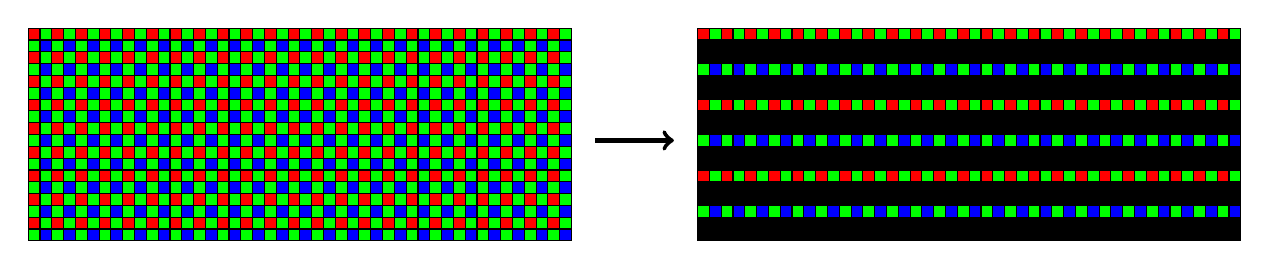
\begin{tikzpicture}

\def\pixelSize{1.5mm}
% 3:2, starting from 0
\def\pixelsX{45}
\def\pixelsY{17}

\def\scenePad{1.6cm}

\newcommand*{\pixelrow}[3] {
	\foreach \x in {0,2,...,\pixelsX}{
		\draw [black,fill=#2] ({\x*\pixelSize},-{#1*\pixelSize}) rectangle ++(\pixelSize,\pixelSize);
	}
	\foreach \x in {1,3,...,\pixelsX}{
		\draw [black,fill=#3] ({\x*\pixelSize},-{#1*\pixelSize}) rectangle ++(\pixelSize,\pixelSize);
	}
}

\foreach \y in {0,2,...,\pixelsY} {
	\pixelrow{\y}{red}{green}
}
\foreach \y in {1,3,...,\pixelsY} {
	\pixelrow{\y}{green}{blue}
}

\draw [->,ultra thick] (\pixelsX*\pixelSize+\pixelSize+0.3cm,-0.5*\pixelsY*\pixelSize) -- ++(1.0cm, 0);

\begin{scope}[xshift = \pixelsX*\pixelSize+\pixelSize+\scenePad]
	\foreach \y in {0,6,...,\pixelsY} {
		\pixelrow{\y}{red}{green}
	}
	\foreach \y in {1,7,...,\pixelsY} {
		\pixelrow{\y}{black}{black}
	}
	\foreach \y in {2,8,...,\pixelsY} {
		\pixelrow{\y}{black}{black}
	}
	\foreach \y in {3,9,...,\pixelsY} {
		\pixelrow{\y}{green}{blue}
	}
	\foreach \y in {4,10,...,\pixelsY} {
		\pixelrow{\y}{black}{black}
	}
	\foreach \y in {5,11,...,\pixelsY} {
		\pixelrow{\y}{black}{black}
	}
\end{scope}

\end{tikzpicture}
\end{document}

